\documentclass[sigconf]{acmart}

\usepackage{xspace}
\usepackage{graphics}
\usepackage[T1]{fontenc}
\usepackage{times}
\usepackage{color}
\usepackage{booktabs}
\usepackage{textcomp}
\usepackage{microtype}
\usepackage{ccicons}
\usepackage{todonotes}
\usepackage{amsthm}
\usepackage{amsmath}
\usepackage{subcaption}
\usepackage{hyperref}
\usepackage{url}
\usepackage{relsize}
\usepackage{caption}
\usepackage{soul}
\usepackage[normalem]{ulem}
\newtheorem{example}{Example}
\hypersetup{
  colorlinks,
  urlcolor=blue}
\renewcommand*{\UrlFont}{\ttfamily\smaller\relax}

\newcommand{\stepCounter}[1]{{\Large\textcircled{{\small#1}}}}

\AtBeginDocument{%
  \providecommand\BibTeX{{%
    \normalfont B\kern-0.5em{\scshape i\kern-0.25em b}\kern-0.8em\TeX}}%
  \raggedbottom
}
\setcopyright{acmcopyright}
\copyrightyear{2024}
\acmYear{2024}
\acmDOI{XXXXXXX.XXXXXXX}
\acmConference[SIGMOD '24]{International Conference on Management of Data}{June 09--15, 2024}{Santiago, Chile}
\acmPrice{15.00}
\acmISBN{978-1-4503-XXXX-X/18/06}

\setcopyright{none}
\renewcommand\footnotetextcopyrightpermission[1]{}
\settopmatter{printacmref=false}
\acmDOI{}
\acmConference[]{}{}{}
\acmBooktitle{}
\acmISBN{}
\date{}

% Packages needed by the literature-review content
\usepackage{array}
\usepackage{balance}
\usepackage{capt-of}
\usepackage{dblfloatfix}
\usepackage{float}
\usepackage{forest}
\usepackage{makecell}
\usepackage{multirow}
\usepackage{placeins}
\usepackage{ragged2e}
\usepackage{tabularx}
\usepackage{tikz}
\usepackage{xcolor}
\usetikzlibrary{positioning,calc,arrows.meta}

% --- floats (two-column) ---
\setcounter{topnumber}{2}
\setcounter{dbltopnumber}{2}
\renewcommand{\topfraction}{0.9}
\renewcommand{\dbltopfraction}{0.9}
\renewcommand{\textfraction}{0.07}
\renewcommand{\floatpagefraction}{0.85}
\renewcommand{\dblfloatpagefraction}{0.85}

\setlength{\textfloatsep}{8pt plus 2pt minus 2pt}
\setlength{\dbltextfloatsep}{8pt plus 2pt minus 2pt}
\setlength{\floatsep}{6pt plus 2pt minus 2pt}
\setlength{\dblfloatsep}{6pt plus 2pt minus 2pt}
\setlength{\intextsep}{6pt plus 2pt minus 2pt}

% Custom X-like column
\newcolumntype{Y}{>{\RaggedRight\arraybackslash}X}

% One table formatting macro used everywhere
\newcommand{\tbl}{%
  \scriptsize
  \setlength{\tabcolsep}{4pt}%
  \renewcommand{\arraystretch}{1.12}%
}

\begin{document}
\pagestyle{plain}

% ======================
% Title + Authors
% ======================
\title[Survey of Data Discovery to Integration in Data Lakes]%
{From Data Discovery to Analytics-Ready Data:\\A Survey of Search, Preparation, and Integration in Data Lakes}

\author{Sumaiya Azad}
\affiliation{%
  \institution{University of Utah}
  \city{Salt Lake City}
  \state{Utah}
  \country{USA}}
\email{sumaiya.azad@utah.edu}

\renewcommand{\shortauthors}{Azad et al.}


% ======================
% Abstract
% ======================

\begin{abstract}
Organizations collect many kinds of data in data lakes---for example, spreadsheet-like tables, JSON or XML files, server logs, and fields extracted from documents. Before anyone can run queries or build dashboards, teams must (i)~find the right data sources, (ii)~clean and organize them, and (iii)~line up columns and records across sources so they can be combined.

We review 49 methods published from 2022 to 2025 and group them by what they produce across three phases: \emph{Discovery \& Search} (ranked lists of relevant tables for keyword, join, and union queries), \emph{Preparation \& Wrangling} (cleaned tables and reusable processing workflows), and \emph{Integration \& Matching} (column-to-column matches, record-level entity matches, and merged tables). For each phase, we describe common tasks, system designs, and how methods are evaluated. We also trace what is shared across phases---for example, vector representations (called \emph{embeddings}) trained once and reused for both search and matching. We close with open challenges, including end-to-end evaluation, keeping results up to date as data changes, reliable use of language models for data tasks, and more.
\end{abstract}

% ======================
% CCS Concepts (single block)
% ======================
\begin{CCSXML}
<ccs2012>
 <concept>
  <concept_id>10002951.10003260</concept_id>
  <concept_desc>Information systems~Information integration</concept_desc>
  <concept_significance>500</concept_significance>
 </concept>
 <concept>
  <concept_id>10002951.10003260.10003300</concept_id>
  <concept_desc>Information systems~Data cleaning</concept_desc>
  <concept_significance>500</concept_significance>
 </concept>
 <concept>
  <concept_id>10002951.10003260.10003309</concept_id>
  <concept_desc>Information systems~Data exchange</concept_desc>
  <concept_significance>300</concept_significance>
 </concept>
 <concept>
  <concept_id>10002951.10003260.10003305</concept_id>
  <concept_desc>Information systems~Data mining</concept_desc>
  <concept_significance>300</concept_significance>
 </concept>
 <concept>
  <concept_id>10002951.10003260.10003310</concept_id>
  <concept_desc>Information systems~Data retrieval</concept_desc>
  <concept_significance>300</concept_significance>
 </concept>
</ccs2012>
\end{CCSXML}

\ccsdesc[500]{Information systems~Information integration}
\ccsdesc[500]{Information systems~Data cleaning}
\ccsdesc[300]{Information systems~Data exchange}
\ccsdesc[300]{Information systems~Data mining}
\ccsdesc[300]{Information systems~Data retrieval}


\keywords{data lakes, dataset discovery, table search, join discovery, union discovery, data preparation, data wrangling, data cleaning, schema matching, entity resolution, data integration, analytics-ready data}


\maketitle

% ==========================================================
\section{Introduction}
Data lakes store many kinds of data together---spreadsheet-like tables, semi-structured files (such as JSON or XML), server logs, and fields pulled from documents---without requiring one fixed column layout (called a \emph{schema}) at load time.
Loading data is easy, but using it later is hard.
Before analysts can run queries, build dashboards, or train models, they must (1)~find the right data, (2)~clean and organize it, and (3)~combine it from multiple sources.

\paragraph{Scope and terminology.}
\emph{Discovery} means finding relevant tables or columns, including \emph{join} search (tables sharing a key column) and \emph{union} search (tables with compatible columns)~\cite{10.1145/3555041.3589409,10.14778/3750601.3750694}. \emph{Preparation} means cleaning errors, transforming values, and organizing raw data into usable tables or reusable workflows. \emph{Integration} means lining up columns across sources and producing a merged output; \emph{entity resolution (ER)} is the special case of deciding whether two records describe the same real-world thing. We use \emph{analytics-ready data} to mean data clean and structured enough for reports, statistics, or machine learning.

Two trends make this pipeline harder: (1)~modern data lakes are large and weakly documented~\cite{10.1145/3555041.3589409,10.14778/3750601.3750694}; (2)~embedding-based and language-model-based methods now appear in all three stages~\cite{10.14778/3659437.3659461,10.14778/3611540.3611624,10.14778/3742728.3742757}, raising concerns about cost, reliability, and privacy.

This survey follows the full path from raw lake data to analytics-ready outputs in three phases:
(1) \emph{Discovery \& Search} finds relevant tables and ranks candidates that could be joined or unioned;
(2) \emph{Preparation \& Wrangling} cleans, restructures, and transforms selected data into usable tables or reusable automated workflows; and
(3) \emph{Integration \& Matching} lines up columns and records across sources to produce a single merged dataset.
We describe our six-step process for selecting and organizing methods in Section~\ref{sec:methodology}.

Our main focus is the connection among these three phases. Instead of treating discovery, preparation, and integration as separate tasks, we study them as one pipeline where each stage feeds the next.

\paragraph{Contributions.}
\begin{itemize}
  \item We review 49 methods published from 2022 to 2025 in three top database venues (SIGMOD, PVLDB, and ICDE) using a clear process for selecting and categorizing methods (Section~\ref{sec:methodology}).
  \item We propose a taxonomy that groups methods by what they produce---ranked candidate lists, cleaned tables, automated workflows, column matches, or merged datasets---spanning discovery, preparation, and integration (Section~\ref{sec:taxonomy-classes}).
  \item We summarize the tasks, system designs, and evaluation practices in each phase, including trade-offs between effectiveness, cost, and the need for human oversight (Section~\ref{sec:pubs-by-phase}).
  \item We identify open problems, including pipeline-level evaluation, keeping results up to date as data changes, reliable use of language models, fairness and privacy constraints, and the need for shared test collections (Section~\ref{sec:discussion-challenges}).
\end{itemize}


% ==========================================================
\section{Related Work}
\label{sec:related}
Earlier surveys cover \emph{discovery} in data lakes in depth, including keyword search, join discovery (finding tables that share a key column), union discovery (finding tables with compatible columns), indexing (building lookup structures for fast search), and benchmarking (standardized tests for comparing methods) \cite{10.1145/3555041.3589409,10.14778/3750601.3750694}. These surveys clearly define the main discovery tasks and compare systems in detail.

Other work studies individual tasks such as \emph{data cleaning} (fixing errors and inconsistencies), \emph{schema matching} (deciding which columns in two tables refer to the same concept), and \emph{entity resolution} (deciding whether two records describe the same real-world thing) \cite{10.14778/3675034.3675051,10.14778/3742728.3742757,10.1145/3588722}. However, most of these methods focus on one stage at a time and assume data is already somewhat organized. They usually do not show how one stage's output feeds into the next stage in a lake pipeline.

Our survey differs in three ways. First, we assign each method to exactly one phase based on its main output (Section~\ref{sec:methodology}), which avoids double-counting and makes comparisons clearer. Second, we connect discovery, preparation, and integration in one view, showing how each stage depends on the others. Third, we focus on 2022--2025, which lets us capture recent language-model-based methods, newer system designs, and emerging concerns such as cost, reliability, fairness, and privacy.


% ==========================================================
\section{Methodology}
\label{sec:methodology}
This section explains how we found, selected, and organized the methods in this survey, with enough detail to reproduce the search and check inclusion decisions.

\paragraph{Step 1: Research questions.}
For each method we ask four questions: (i)~which phase does it target (discovery, preparation, or integration)? (ii)~what does it mainly produce (for example, a ranked list, a cleaned table, or a merged dataset)? (iii)~what technique does it use? and (iv)~how is it evaluated (which datasets, which metrics, and whether cost is reported)?

\paragraph{Step 2: Search terms.}
We search using the query \texttt{"data lake" AND (S1 OR S2 OR S3 OR S4)}, where S1 through S4 are groups of task-related keywords listed in Table~\ref{tab:search-strings}.


% ---------- Table: Search terms ----------
\begin{table}[!htbp]
\caption{Search term groups used for queries over data lakes.}
\label{tab:search-strings}
\centering
\tbl
\begin{tabularx}{\columnwidth}{@{}p{8mm}X@{}}
\toprule
\textbf{ID} & \textbf{Query family (examples of task keywords)} \\
\midrule
S1 & \texttt{discovery}, \texttt{search}, \texttt{table search}, \texttt{dataset retrieval}, \texttt{exploration} \\
S2 & \texttt{joinable}, \texttt{unionable}, \texttt{overlap}, \texttt{join discovery}, \texttt{union discovery} \\
S3 & \texttt{wrangling}, \texttt{preparation}, \texttt{cleaning}, \texttt{transform}, \texttt{pipeline synthesis} \\
S4 & \texttt{schema matching}, \texttt{entity resolution}, \texttt{record linkage}, \texttt{data integration}, \texttt{LLM} \\
\bottomrule
\end{tabularx}
\end{table}

\paragraph{Step 3: Sources and retrieval.}
We scan proceedings of three top database venues---SIGMOD, PVLDB, and ICDE---by running title and abstract queries with the keyword groups S1--S4.
The final collection includes 49 methods: 15 from SIGMOD, 22 from PVLDB, and 12 from ICDE.

\paragraph{Step 4: Inclusion and exclusion.}
We include methods that study a data lake or lakehouse setting and that propose a concrete technique for discovery, preparation, or integration. We exclude methods that do not target a lake setting.

\paragraph{Step 5: Coding rule.}
Each method is assigned to exactly one phase based on its \emph{primary output}---the main thing it produces. Specifically: a method that outputs a ranked list of candidate tables goes into Discovery; a method that outputs a cleaned table, transformed data, or a reusable processing workflow goes into Preparation; and a method that outputs column matches, record-level entity matches, or a merged dataset goes into Integration. This rule prevents double-counting and makes the taxonomy clear.

\paragraph{Step 6: Synthesis.}
We group all 49 methods by the taxonomy defined in Section~\ref{sec:taxonomy-classes} and summarize the distribution across phases in Table~\ref{tab:taxonomy-summary}. The later literature-review sections describe techniques and evaluation practices within each category.

% ---------- Table: Top-level distribution ----------
\begin{table}[!htbp]
  \caption{Top-level taxonomy distribution.}
  \label{tab:taxonomy-summary}
  \centering
  \tbl
  \begin{tabular}{lr}
    \toprule
    Category & \# Methods \\
    \midrule
    Discovery and Search & 19 \\
    Preparation and Wrangling & 13 \\
    Integration and Matching & 17 \\
    \midrule
    Total & 49 \\
    \bottomrule
  \end{tabular}
\end{table}


\section{Taxonomy Overview}

We organize the 49 methods into a two-level taxonomy. The top level has three \emph{classes}, one for each phase of the pipeline (Discovery, Preparation, Integration). Within each class, we define \emph{categories} that capture common method patterns---for example, ``cleaning and repair'' is one category inside the Preparation class.


% ----------------------------------------------------------
\subsection{Classification Summary}

% ---------- Compact taxonomy diagram ----------
\begin{figure*}[t]
\centering
\scriptsize
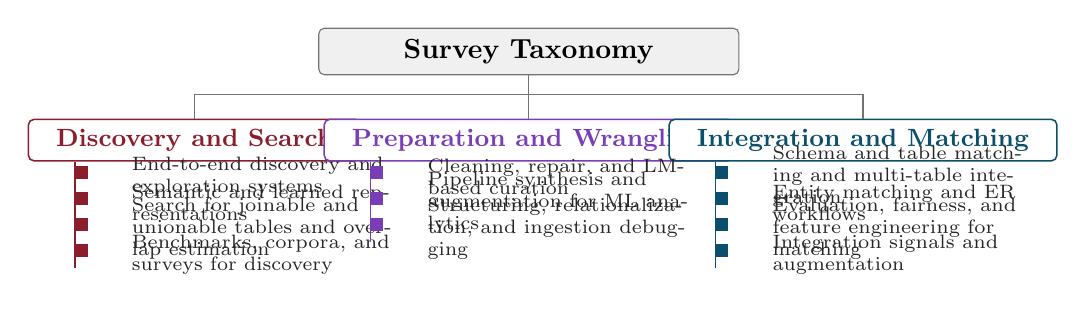
\begin{tikzpicture}[
  font=\scriptsize,
  >=Latex,
  conn/.style={draw=black!55, line width=0.45pt},
  title/.style={draw=black!55, rounded corners=2pt, fill=black!6,
                inner xsep=10pt, inner ysep=4pt, align=center,
                minimum width=0.44\textwidth},
  cat/.style={rounded corners=2pt, fill=white,
              inner xsep=10pt, inner ysep=3.5pt, align=center,
              minimum width=0.26\textwidth, line width=0.55pt},
  itemtext/.style={anchor=west, text=black!85, text width=0.27\textwidth}
]

% Colors
\definecolor{discC}{HTML}{8B1E2D}
\definecolor{prepC}{HTML}{7A3DB8}
\definecolor{inteC}{HTML}{0B4F6C}

% Bullet square size
\def\bs{1.6mm}

\def\gapTop{5.5mm}
\def\barDrop{2.4mm}
\def\stem{2.2mm}
\def\ygap{3.3mm}
\def\xoff{6.0mm}
\def\spineInset{6mm}

% --- Top title ---
\node[title] (root) {\textbf{\normalsize Survey Taxonomy}};

% --- Phase boxes ---
\node[cat, draw=discC, text=discC, below=\gapTop of root, xshift=-0.35\textwidth] (disc)
  {\textbf{\small Discovery and Search}};
\node[cat, draw=prepC, text=prepC, below=\gapTop of root] (prep)
  {\textbf{\small Preparation and Wrangling}};
\node[cat, draw=inteC, text=inteC, below=\gapTop of root, xshift= 0.35\textwidth] (inte)
  {\textbf{\small Integration and Matching}};

% --- Connector bar ---
\coordinate (barC) at ($(root.south)+(0,-\barDrop)$);
\coordinate (barL) at ($(disc.north |- barC)$);
\coordinate (barR) at ($(inte.north |- barC)$);

\draw[conn] (root.south) -- (barC);
\draw[conn] (barL) -- (barR);
\draw[conn] (barL) -- (disc.north);
\draw[conn] (barC) -- (prep.north);
\draw[conn] (barR) -- (inte.north);

% ---------- Discovery ----------
\coordinate (discStem) at ($(disc.south west)+(\spineInset,0)$);
\coordinate (discB1)   at ($(discStem)+(0,-\stem)$);
\coordinate (discB2)   at ($(discB1)+(0,-\ygap)$);
\coordinate (discB3)   at ($(discB2)+(0,-\ygap)$);
\coordinate (discB4)   at ($(discB3)+(0,-\ygap)$);

\draw[conn, draw=discC] (discStem) -- ($(discB4)+(0,-1.4mm)$);

\foreach \p/\txt in {
  discB1/{End-to-end discovery and exploration systems},
  discB2/{Semantic and learned representations},
  discB3/{Search for joinable and unionable tables and overlap estimation},
  discB4/{Benchmarks, corpora, and surveys for discovery}
}{
  \fill[discC] (\p) rectangle ++(\bs,\bs);
  \node[itemtext] at ($(\p)+(\xoff,0.3mm)$) {\txt};
}

% ---------- Preparation ----------
\coordinate (prepStem) at ($(prep.south west)+(\spineInset,0)$);
\coordinate (prepB1)   at ($(prepStem)+(0,-\stem)$);
\coordinate (prepB2)   at ($(prepB1)+(0,-\ygap)$);
\coordinate (prepB3)   at ($(prepB2)+(0,-\ygap)$);

\draw[conn, draw=prepC] (prepStem) -- ($(prepB3)+(0,-1.4mm)$);

\foreach \p/\txt in {
  prepB1/{Cleaning, repair, and LM-based curation},
  prepB2/{Pipeline synthesis and augmentation for ML analytics},
  prepB3/{Structuring, relationalization, and ingestion debugging}
}{
  \fill[prepC] (\p) rectangle ++(\bs,\bs);
  \node[itemtext] at ($(\p)+(\xoff,0.3mm)$) {\txt};
}

% ---------- Integration ----------
\coordinate (inteStem) at ($(inte.south west)+(\spineInset,0)$);
\coordinate (inteB1)   at ($(inteStem)+(0,-\stem)$);
\coordinate (inteB2)   at ($(inteB1)+(0,-\ygap)$);
\coordinate (inteB3)   at ($(inteB2)+(0,-\ygap)$);
\coordinate (inteB4)   at ($(inteB3)+(0,-\ygap)$);

\draw[conn, draw=inteC] (inteStem) -- ($(inteB4)+(0,-1.4mm)$);

\foreach \p/\txt in {
  inteB1/{Schema and table matching and multi-table integration},
  inteB2/{Entity matching and ER workflows},
  inteB3/{Evaluation, fairness, and feature engineering for matching},
  inteB4/{Integration signals and augmentation}
}{
  \fill[inteC] (\p) rectangle ++(\bs,\bs);
  \node[itemtext] at ($(\p)+(\xoff,0.3mm)$) {\txt};
}

\end{tikzpicture}
\caption{Taxonomy of data lake research from discovery and search to analytics-ready outputs via preparation and integration.}
\label{fig:taxonomy}
\end{figure*}


Figure~\ref{fig:taxonomy} shows the three classes and their categories. Together, they reflect the common path from raw lake contents to analytics-ready outputs.

\textbf{Discovery and Search} returns ranked lists of candidate data sources---individual tables, specific columns, or derived views (tables created on-the-fly by joining or filtering existing tables, as in Ver~\cite{10184768})---that help analysts decide what to use next \cite{10184768,10.14778/3681954.3682005}. Systems in this phase must work with incomplete metadata (for example, missing column descriptions) and handle large-lake challenges such as keeping search indexes fast and up to date. Recent methods combine meaning-based vector representations, indexes, and search operators to support keyword search and finding joinable or unionable candidates. The actual merge happens later, in the integration phase. Representative methods include LakeCompass~\cite{10.14778/3685800.3685880}, CHORUS~\cite{10.14778/3659437.3659461}, and BLEND~\cite{11112882}.

\textbf{Preparation and Wrangling} returns cleaned, reorganized, or transformed datasets---for example, tables with dates converted to a standard format, or new columns added by computation. This phase also increasingly produces \emph{reusable automated workflows}: step-by-step processing scripts that can run again when new data arrives, instead of one-time manual fixes. We group preparation methods into three categories: cleaning and repair, building automated pipelines for machine-learning analytics, and converting messy inputs (such as nested JSON files) into well-structured tables. Representative methods include CtxPipe~\cite{10.1145/3698831} and CM Explorer~\cite{10.14778/3611540.3611595}.

\textbf{Integration and Matching} returns alignment results and merged outputs. For example, it may determine that \texttt{zip\_code} in one table means the same thing as \texttt{postal\_code} in another (a \emph{column match}), or that two records with slightly different names refer to the same person (an \emph{entity match}). The final output is a single combined table. This class includes schema matching (lining up columns), entity resolution (linking records), and end-to-end workflows that connect discovery, alignment, and merging into one pipeline. Representative methods include FlexER~\cite{10.1145/3588722}, DIALITE~\cite{10.1145/3555041.3589732}, Magneto~\cite{10.14778/3742728.3742757}, and PLM Schema Matching~\cite{10184612}.


\subsection{Classes and Their Categories}
\label{sec:taxonomy-classes}
Below, we define each class and its categories. For each class, we state what it produces, then describe the recurring tasks and the kinds of methods we found. The full category breakdown is shown in Figure~\ref{fig:taxonomy}.

In \textbf{Discovery and Search}, methods cluster around four areas: (1)~end-to-end discovery systems that combine indexing and search in one stack, (2)~learned representations (vector embeddings that capture column or table meaning), (3)~search for joinable and unionable candidates (finding tables that can be linked or stacked), and (4)~shared benchmarks and \emph{corpora}---large publicly available table collections, such as GitTables~\cite{10.1145/3588710}, that researchers use to train models and compare results on a common footing.

In \textbf{Preparation and Wrangling}, the categories are: (1)~cleaning and repair (fixing errors and inconsistencies), (2)~pipeline construction for analytics (building automated step-by-step workflows that prepare data for machine learning), and (3)~structuring heterogeneous inputs and debugging ingestion---that is, converting messy files into clean relational tables and diagnosing errors that happen when data is first loaded into the lake.

In \textbf{Integration and Matching}, the categories are: (1)~schema and table matching (lining up columns across tables and merging them), (2)~entity-resolution workflows (deciding which records refer to the same real-world entity), (3)~fairness-aware evaluation (checking whether matching errors are distributed unevenly across demographic groups), and (4)~reusable integration signals (lightweight evidence, such as approximate foreign-key relationships, that can be shared across tasks).

\begin{table*}[!htbp]
\centering
\caption{Survey summary by phase: outputs, recurring tasks, and typical concerns.}
\label{tab:phase-summary}
\tbl
\begin{tabularx}{\textwidth}{@{}p{30mm}p{34mm}Y p{42mm}@{}}
\toprule
\textbf{Phase} & \textbf{Primary output} & \textbf{Recurring tasks} & \textbf{Typical concerns} \\
\midrule
Discovery \& Search &
Ranked candidate tables, columns, views, or augmentations &
Keyword search, joinable and unionable table search, overlap estimation (how much two tables share), interactive exploration, and benchmark construction &
Weak metadata, retrieval quality in large lakes, index maintenance (keeping indexes updated as data changes), and ambiguity during exploration \\
\addlinespace[0.25em]
Preparation \& Wrangling &
Cleaned tables, structured views, changed tables (e.g., standardized dates or added derived columns), or rerunnable workflows &
Repair, transformation recommendation, pipeline synthesis, feature augmentation (adding useful columns), relationalization, and ingestion debugging &
Do-no-harm behavior, repeatability, downstream utility, validation hooks, and changing data conditions \\
\addlinespace[0.25em]
Integration \& Matching &
Column matches (e.g., \texttt{zip\_code} = \texttt{postal\_code}), entity matches or clusters, reusable DI signals, and merged datasets &
Schema matching, entity resolution, filtering and scheduling, augmentation, dependency discovery, and merge rules (\emph{integration semantics}: rules for how partial rows are combined) &
Intent ambiguity, supervision cost, completeness and consistency of outputs, fairness, privacy, and policy constraints \\
\bottomrule
\end{tabularx}
\end{table*}

% ----------------------
\subsubsection{Discovery and Search}
\paragraph{Output.} A ranked list of candidate data sources (tables, columns, or derived views) for the analyst to explore, join, or union.

End-to-end systems combine background work such as profiling tables and keeping indexes up to date with real-time search and interactive exploration \cite{10.14778/3685800.3685880,11112882,10.14778/3659437.3659461}.
Representation methods learn compact vector embeddings or statistical sketches for columns and tables, so that search can rely on meaning rather than exact text matches, even when metadata is missing or inconsistent \cite{10.14778/3587136.3587146,11113165,11113110}.
Join search, union search, and overlap estimation find candidate tables that share data with a given seed table, then score how strongly each candidate is related \cite{10.14778/3603581.3603587,10.1145/3588689,10.1145/3725365}. These are discovery-time steps: they identify candidates but do not produce the final merged table.
Benchmarks and corpora (large shared table collections such as GitTables~\cite{10.1145/3588710}) support fair comparison and model training at lake scale \cite{10.14778/3659437.3659448}.


% ----------------------
\subsubsection{Preparation and Wrangling}
\paragraph{Output.} Cleaned or transformed tables, well-structured relational views (standard row-and-column tables), and reusable automated workflows that can run again when new data arrives.

Cleaning and language-model-based curation methods study how to fix errors, reduce data quality problems, and build reusable cleaning workflows---for example, a pipeline that detects and corrects misspelled city names \cite{10.14778/3675034.3675051,10.14778/3574245.3574258,10.14778/3611540.3611624,10.14778/3611540.3611628}.
Pipeline synthesis methods search for the best sequence of processing steps (such as removing duplicates, then standardizing dates, then adding a computed column) that improve results for a downstream task like training a classifier \cite{10.1145/3698831,10.1145/3588945,11113027,10.14778/3603581.3603596}.
Structuring and ingestion debugging methods convert messy inputs (such as nested JSON files or inconsistent spreadsheets) into clean relational tables, and help diagnose errors that occur when data is first loaded into the lake \cite{10.14778/3626292.3626294,10.1145/3665252.3665269,10.14778/3681954.3682019,10.14778/3611540.3611595}.


% ----------------------
\subsubsection{Integration and Matching}
\paragraph{Output.} Column matches (for example, determining that \texttt{zip\_code} in one table means the same as \texttt{postal\_code} in another), entity matches or clusters (groups of records that refer to the same entity), and merged datasets.

Schema and table integration methods line up columns across multiple tables and apply explicit merge rules---called \emph{integration semantics}---that specify, for instance, how to fill in missing values when different sources each provide only part of the information \cite{10.1145/3555041.3589732,10.14778/3574245.3574274,10.14778/3742728.3742757,10184612}.
Entity-resolution (ER) workflows combine three steps: \emph{blocking} (quickly eliminating obviously non-matching pairs to reduce comparisons), \emph{matching} (scoring how likely two records are to be the same entity), and \emph{clustering} (grouping matched records together). These workflows must balance labeling cost against accuracy \cite{10.1145/3709715,10.1145/3588722,10.1145/3588712,10.1145/3626711,10.1145/3588938}.
Evaluation work studies how to trade off speed versus quality in filtering, whether error rates differ across demographic subgroups (fairness), and how to build useful matching features at low cost \cite{10184692,10.14778/3611479.3611525,11112979,10.14778/3681954.3681987}.
Other methods produce reusable signals---such as approximate foreign-key relationships, shared embeddings, and selectively retrieved external data---that can help multiple integration tasks at once \cite{10.1145/3588929,10184556,10.14778/3611479.3611535,10.14778/3603581.3603602}.

These three classes form a single pipeline: discovery narrows a lake to candidates, preparation converts them into stable outputs, and integration produces the final merged result.



% ==========================================================
\section{Literature Review}
% ==========================================================

% ----------------------
\subsection{Discovery and Search}
Discovery and search form the entry point of the lake-to-analytics pipeline. Imagine a data lake with thousands of tables, many lacking descriptions or consistent column names. An analyst looking for customer-address data must somehow find the right tables among all of these. Discovery methods help by surfacing a small, ranked set of relevant data sources for exploration or enrichment. In the methods we reviewed, discovery usually combines three ingredients: understanding what tables contain, retrieving the most relevant ones, and letting users interact to refine results. Table~\ref{tab:discovery-methods} summarizes this phase by category, keywords, and one-line contribution.

\begin{table*}[!htbp]
\caption{Discovery \& Search methods mapped to taxonomy.}
\label{tab:discovery-methods}
\tbl
\begin{tabularx}{\textwidth}{@{}p{24mm}p{28mm}p{18mm}Y@{}}
\toprule
\textbf{Category} & \textbf{Reference} & \textbf{Keywords} & \textbf{Contribution (one line)} \\
\midrule

End-to-end discovery and exploration systems &
CHORUS~\cite{10.14778/3659437.3659461} &
LM, annotation &
Unifies multiple lake discovery/exploration tasks with a foundation-model pipeline and reports consistent gains over task-specific baselines. \\

~ &
BLEND~\cite{11112882} &
plans, ranking &
Defines a declarative discovery-plan abstraction that compiles to improved execution over heterogeneous signals for unified keyword, join, and union discovery with top-$k$ retrieval. \\

~ &
LakeCompass~\cite{10.14778/3685800.3685880} &
indexing, workflows &
End-to-end lake stack for maintenance + search + analysis workflows, with scalable indexing and practical lake operations. \\

~ &
METAM~\cite{10184845} &
utility, ranking &
Ranks candidate datasets by expected downstream task utility (goal-aware profiling + ranking). \\

~ &
Selecting Sub-tables~\cite{10184535} &
sampling, previews &
Selects compact, informative sub-tables to accelerate inspection when full tables are too large or noisy. \\

~ &
Ver~\cite{10184768} &
views, interaction &
Question-driven view discovery that progressively prunes the space to surface useful derived tables. \\

\midrule

Semantic and learned representations &
CMDL~\cite{10.14778/3611479.3611533} &
cross-modal, embeddings &
Learns joint representations to retrieve across structured tables and unstructured text sources for cross-modal dataset discovery. \\

~ &
Starmie~\cite{10.14778/3587136.3587146} &
embeddings, contrastive &
Pretrains contextualized column representations that capture table context to improve semantic dataset discovery, especially unionable-table retrieval. \\

~ &
LIFTus~\cite{11113165} &
fusion, columns &
Learns multi-aspect column representations and adaptively fuses them to boost union search quality across heterogeneous lakes. \\

~ &
TabSketchFM~\cite{11113110} &
sketches, tokens &
Uses compact column sketches with a pretrained tabular model to scale discovery under token/compute constraints. \\

\midrule

Search for joinable and unionable tables and overlap estimation &
DeepJoin~\cite{10.14778/3603581.3603587} &
joinability, retrieval &
PLM-based joinable-table discovery that embeds columns to rank candidate join partners, improving join discovery over lexical baselines. \\

~ &
SANTOS~\cite{10.1145/3588689} &
unionability, semantics &
Relationship-aware semantic union search using relational/context signals to find unionable tables with compatible meaning. \\

~ &
Nested/Joined Lake Search~\cite{10.14778/3681954.3682005} &
nested, joins &
Extends lake search to nested and join-derived candidates not well-modeled as flat standalone tables. \\

~ &
Armadillo~\cite{10.1145/3725365} &
overlap, graphs &
Learns table embeddings whose similarity approximates overlap ratio for fast scalable overlap estimation. \\

\midrule

Benchmarks, corpora, and surveys for discovery &
Rottnest~\cite{11113229} &
indexing, search &
Scalable lake indexing techniques to support efficient search over large, evolving lakes. \\

~ &
GitTables~\cite{10.1145/3588710} &
corpus, benchmark &
Large public corpus of relational tables mined at scale for reproducible training and evaluation. \\

~ &
LakeBench~\cite{10.14778/3659437.3659448} &
benchmark, labels &
Benchmark suite for joinable and unionable table discovery with ground-truth labeling at lake scale. \\

~ &
Data Discovery Survey~\cite{10.14778/3750601.3750694} &
survey, taxonomy &
Consolidates discovery operations (indexes + systems) and evaluation practice, noting gaps in workloads and cost reporting. \\

~ &
Table Discovery Survey~\cite{10.1145/3555041.3589409} &
survey, methods &
Consolidated overview of table discovery methods and open directions at lake scale. \\

\bottomrule
\end{tabularx}
\end{table*}

Four patterns emerge. First, systems are moving from single search features to end-to-end stacks that handle indexing, search, and user interaction together. Second, retrieval quality increasingly depends on learned embeddings rather than metadata alone. Third, join search, union search, and overlap estimation serve as building blocks for later integration. Fourth, shared corpora and benchmarks are essential for fair comparison.

\subsubsection{End-to-end Discovery and Exploration Systems}
End-to-end discovery systems return ranked tables, derived views, or dataset augmentations. A common architecture has three parts: (i)~offline enrichment (profiling, indexing); (ii)~online retrieval (keyword, join, union, and view search); and (iii)~interactive exploration.

\paragraph{Foundation models as a shared backbone for discovery.}
CHORUS~\cite{10.14778/3659437.3659461} uses a large language model (a ``foundation model'') to produce shared understanding of each table---for example, detecting what category a table belongs to, what type each column is, and which columns could be used to join tables together. These annotations are then reused for indexing, filtering, and ranking.

Because one model drives several tasks, signals can be reused efficiently. However, this also means that prompt sensitivity (small wording changes leading to different answers), non-determinism (the model giving different outputs on repeated runs), and cost can affect multiple decisions at once.

\paragraph{Unifying discovery operators with declarative plans.}
BLEND~\cite{11112882} makes the discovery pipeline explicit and tunable by introducing \emph{discovery plans}---multi-step workflows written in a declarative style (the user states \emph{what} to find, not \emph{how}). Each plan mixes retrieval, composition, and ranking steps, connecting offline indexes to real-time execution and letting the system choose efficient orderings automatically.

\paragraph{Operational stacks that couple maintenance, search, and analysis.}
LakeCompass~\cite{10.14778/3685800.3685880} packages the full pipeline as a single system: it manages table storage and multiple index structures, supports keyword, join, and union search, and exposes results through APIs and an interactive exploration interface.

\paragraph{Goal-oriented discovery via downstream utility.}
METAM~\cite{10184845} lets the downstream task steer discovery. Instead of ranking candidates only by how similar or joinable they are, METAM checks which candidates actually improve the target analysis (for example, a classifier's accuracy) and uses that improvement as feedback.

\paragraph{Efficient exploration via informative table previews.}
Even when search returns relevant candidates, a table with millions of rows is hard to inspect directly. Selecting Sub-tables~\cite{10184535} addresses this by choosing compact, informative sub-tables---small representative slices of the data---that let analysts quickly decide whether a candidate is worth using.

\paragraph{Interaction under ambiguity: view discovery and narrowing.}
Ver~\cite{10184768} studies \emph{view discovery}: when many ways of joining tables are possible, it searches candidate join structures, removes redundant options, and asks the user targeted questions to narrow down to the intended merged view.

\subsubsection{Semantic and Learned Representations for Discovery}
Because meaning is rarely written down explicitly in data lakes, many methods learn compact embeddings for columns and tables so that search can compare meaning rather than exact text.

\paragraph{Cross-modal embeddings for discovery beyond tables.}
CMDL~\cite{10.14778/3611479.3611533} handles lakes that contain both structured tables and unstructured text documents. It embeds columns and documents into a shared vector space so that, for example, a text report mentioning ``revenue'' can be retrieved alongside a table with a ``revenue'' column. Because labeled cross-modal examples are scarce, CMDL uses weak supervision---automatically generated, approximate labels---to create enough training data.

\paragraph{Contextualized column representations for semantic union search.}
Starmie~\cite{10.14778/3587136.3587146} learns \emph{contextualized} column embeddings: each column's vector reflects not only its own values but also the other columns in the same table. For example, a ``Name'' column next to ``Salary'' and ``Department'' is understood differently from a ``Name'' column next to ``Species'' and ``Habitat.'' The method uses self-supervised contrastive pretraining (learning by comparing positive and negative column pairs) and retrieves candidates via nearest-neighbor search in embedding space.

\paragraph{Multi-aspect representations for heterogeneous columns.}
LIFTus~\cite{11113165} addresses the fact that many lake columns are not well-modeled as natural language---for example, columns of numeric IDs, patterned strings like phone numbers, or physical measurements. It encodes each column through multiple \emph{aspects} (value distribution, data type, textual content) using specialized encoders, then fuses them into a single vector for indexing and search.

\paragraph{Sketch-based neural representations under token and cost constraints.}
TabSketchFM~\cite{11113110} avoids the cost of converting entire tables into text (which can exceed the input limits of language models) by compressing each table into a compact statistical sketch that preserves key similarity signals. A transformer model is trained to read these sketches directly and produce embeddings for efficient retrieval.

\subsubsection{Join and Union Search, and Overlap Estimation}
Join search, union search, and overlap estimation are tightly connected building blocks for \emph{table enrichment}---the process of adding useful rows or columns to a starting table. Given a \emph{seed table} (the analyst's starting point), systems retrieve a small set of candidates that can be joined (linked by a shared key) or unioned (stacked because they have compatible columns), then score how strongly each candidate relates to the seed. This is still discovery: the system identifies candidates but does not yet produce a final merged table.

\paragraph{Joinability and learned retrieval.}
DeepJoin~\cite{10.14778/3603581.3603587} encodes columns into fixed-length vectors using a pre-trained language model fine-tuned on examples of valid joins, then retrieves the top-$k$ join partners using approximate nearest-neighbor (ANN) indexing. This makes join discovery fast even in very large lakes and robust to spelling variations and formatting differences.

\paragraph{Unionability as relational semantic compatibility.}
SANTOS~\cite{10.1145/3588689} models unionability by looking at semantic relationships between columns---for example, whether columns in two tables represent the same concepts (such as ``city'' and ``state'' appearing together). It draws on external knowledge bases or a knowledge base synthesized from the lake itself to distinguish genuine union candidates from tables that merely share surface-level text overlap.

\paragraph{Compositional candidates beyond base tables.}
Nested/Joined Lake Search~\cite{10.14778/3681954.3682005} goes beyond searching for individual tables. It produces and ranks \emph{join-nest candidates}---new tables built on-the-fly by joining and restructuring existing tables---so that search results can match a user's structural intent even when no single base table does.

\paragraph{Overlap as the shared scoring primitive.}
Armadillo~\cite{10.1145/3725365} provides a unifying relatedness measure that works regardless of whether the downstream action is join, union, or deduplication. It formalizes \emph{overlap}---how much data two tables share---and learns graph-based embeddings whose vector similarity approximates overlap at scale.

\subsubsection{Benchmarks, Corpora, and Surveys for Discovery}
Discovery at lake scale depends on shared resources---corpora for training, benchmarks for fair comparison, and indexing techniques for efficient search.

\paragraph{Indexing for heterogeneous search workloads.}
Rottnest~\cite{11113229} proposes a lakehouse indexing protocol that manages the overhead of building and updating indexes, making search-oriented discovery practical on evolving lake storage.

\paragraph{Corpora for learned discovery.}
GitTables~\cite{10.1145/3588710} curates a large corpus of relational-style tables (extracted from GitHub repositories) with semantic-type annotations, supporting both representation learning and table-understanding research.

\paragraph{Benchmarks for join and union discovery.}
LakeBench~\cite{10.14778/3659437.3659448} provides labeled ground-truth queries paired with workloads that test both retrieval quality and system efficiency, enabling fair comparison of discovery methods.

\paragraph{Operations and indexes perspective.}
The Data Discovery Survey~\cite{10.14778/3750601.3750694} gives an operations-focused view of the field and highlights two common gaps: mismatched evaluation setups across studies and weak reporting of computational cost.

\paragraph{Consolidated overview of table discovery methods.}
The Table Discovery Survey~\cite{10.1145/3555041.3589409} synthesizes existing discovery techniques and open research directions, treating robustness and efficiency as first-class concerns.

Once candidate data sources are surfaced, the next phase focuses on transforming these often-messy results into clean, well-structured inputs that can be used for analytics and downstream integration.


% ----------------------
\subsection{Preparation and Wrangling}
% ----------------------

Preparation and wrangling convert the candidates found during discovery into clean, well-organized data that is ready for analysis. While discovery produces a ranked list of candidate tables, preparation actually changes the data. It usually returns one of three things: (i)~a cleaned or repaired dataset (for example, a table with typos fixed and missing values filled in), (ii)~a transformed table with new derived columns (for example, adding a ``full address'' column by combining street, city, and zip code), or (iii)~an automated workflow---a reusable script or pipeline that can run again whenever new data arrives, instead of requiring manual work each time. Table~\ref{tab:prep-methods} groups preparation methods into three categories: (1)~cleaning and repair using language models, (2)~pipeline synthesis and feature augmentation for machine-learning analytics, and (3)~structuring, relationalization (converting messy formats into standard row-and-column tables), and ingestion debugging (finding and fixing errors that occur when data is first loaded).

\begin{table*}[!htbp]
\caption{Preparation \& Wrangling methods mapped to taxonomy.}
\label{tab:prep-methods}
\tbl
\begin{tabularx}{\textwidth}{@{}p{24mm}p{28mm}p{18mm}Y@{}}
\toprule
\textbf{Category} & \textbf{Reference} & \textbf{Keywords} & \textbf{Contribution (one line)} \\
\midrule

Cleaning, repair, and LM-based curation &
Automatic Data Repair~\cite{10.14778/3675034.3675051} &
repair, benchmark &
Benchmarks repair algorithms across datasets/error settings, proposes a repair-search strategy, and distills deployment guidelines. \\

~ &
DataRinse~\cite{10.14778/3611540.3611628} &
transforms, mining &
Recommends semantic data-prep transformations by mining data-preparation code repositories to learn reusable transformation patterns. \\

~ &
Foundation Models for Data Tasks~\cite{10.14778/3574245.3574258} &
LM, prompting &
Casts classical cleaning/integration tasks as prompts and evaluates foundation models, noting strong generalization alongside privacy and domain-specific limitations. \\

~ &
Lingua Manga~\cite{10.14778/3611540.3611624} &
LLM, templates &
Provides a language-model-based curation system with modular templates and orchestration to run end-to-end curation workflows. \\

\midrule

Pipeline synthesis and augmentation for ML analytics &
CtxPipe~\cite{10.1145/3698831} &
pipelines, RL &
Constructs preparation pipelines by conditioning operator selection on dataset/task context and using deep RL to search effective pipelines. \\

~ &
HAIPipe~\cite{10.1145/3588945} &
human-AI, reuse &
Combines human- and machine-generated pipelines via enumeration--sampling (with active learning) and uses RL to search improved AI-pipelines. \\

~ &
Featpilot~\cite{11113027} &
features, joins &
Automatically augments tabular datasets with useful additional features from joinable sources to improve downstream model performance. \\

~ &
Auto-BI~\cite{10.14778/3603581.3603596} &
BI, joins &
Predicts BI schema graphs (joins) via global search, evaluated on large collections of BI models. \\

\midrule

Structuring, relationalization, and ingestion debugging &
Evaporate~\cite{10.14778/3626292.3626294} &
views, synthesis &
Uses language models plus lightweight synthesis and weak supervision to generate structured views over heterogeneous lake inputs. \\

~ &
Auto-Tables~\cite{10.1145/3665252.3665269} &
relationalization, schema &
Relationalizes semi-structured tables without examples by inferring structure/schemas and producing normalized relational output. \\

~ &
ReCG~\cite{10.14778/3681954.3682019} &
JSON, clustering &
Discovers JSON schemas bottom-up by clustering records and generalizing clusters into schema fragments. \\

~ &
CM Explorer~\cite{10.14778/3611540.3611595} &
validation, debugging &
Disentangles correlated violated conditional unit tests using graph-based exploration to localize ingestion errors. \\

~ &
XDBC~\cite{10.1145/3725294} &
transfer, tuning &
Decomposes data transfer into configurable stages and auto-tunes configurations for heterogeneous systems to improve throughput. \\

\bottomrule
\end{tabularx}
\end{table*}

The common theme is \emph{repeatable automated workflows} instead of one-time manual fixes. Because discovery often retrieves messy data and integration assumes reasonably well-structured inputs, preparation directly affects how well later matching works. If preparation fails to standardize date formats, for example, integration may incorrectly treat matching dates as different values---an impact easy to miss when evaluation only reports local metrics.



\subsubsection{Cleaning, Repair, and LM-based Curation}
Data lakes make classic data-quality problems worse: errors are frequent and come in many forms (typos, missing values, inconsistent formats), and the context needed to understand dirty values is often unavailable. Methods in this category focus on two goals: (i)~\emph{deployable repair} that actually reduces the number of errors in a table (not just edits cells in ways that may introduce new mistakes), and (ii)~\emph{reusable curation workflows} that package cleaning know-how into automated, controllable steps.

Different preparation methods optimize different goals---consistency, net error reduction, or downstream model accuracy---and the automatic data repair study~\cite{10.14778/3675034.3675051} shows why mixing these goals without stating them clearly can be misleading.

\paragraph{Deployment-aware objectives and evaluation.}
Automatic Data Repair~\cite{10.14778/3675034.3675051} argues that repair methods should be evaluated by whether they actually reduce the total number of errors, not just by how many cells they change. It benchmarks repair methods across different datasets and error types and proposes strategies to prevent \emph{incorrect repairs}---situations where the repair itself introduces a new error.

\paragraph{Prompting-based wrangling and its constraints.}
Foundation Models for Data Tasks~\cite{10.14778/3574245.3574258} converts traditional data tasks (cleaning, integration, transformation) into text prompts---for example, ``Fix the errors in this row: [data].'' The study shows that large language models can generalize across many task types, but it also surfaces practical constraints: sending data to a model may expose private information, and the model may not understand domain-specific conventions (such as medical codes or financial formatting).

\paragraph{Reusable LM-based curation workflows.}
Lingua Manga~\cite{10.14778/3611540.3611624} provides a system for building language-model-based curation pipelines. Users compose workflows using modular templates and a small scripting language, then the system orchestrates model calls. Its design reduces cost by minimizing expensive model invocations and supports workflows that can be rerun automatically when new lake data arrives.

\paragraph{Mining semantic transforms from preparation code.}
DataRinse~\cite{10.14778/3611540.3611628} takes a different approach: instead of using a language model, it mines transformation patterns by analyzing existing data-preparation code. It groups related field-level expressions (for example, all ways people have cleaned phone-number columns) so that suggestions remain coherent, and presents them as human-in-the-loop recommendations---the analyst reviews and approves each suggestion before it is applied.



\subsubsection{Pipeline Synthesis and Augmentation for ML Analytics}
Pipeline synthesis treats data preparation as a search problem: given raw tables and a goal (such as training an accurate classifier), the system automatically finds the best sequence of processing steps---cleaning, transforming, and adding features---that improves the final result within a given budget.

\paragraph{Context-conditioned pipeline construction.}
CtxPipe~\cite{10.1145/3698831} addresses the problem that the space of possible processing steps is enormous (hundreds of operator combinations). It uses dataset characteristics and task feedback to narrow down which operators to try first, prioritizing transformations that are more likely to improve the downstream model.

\paragraph{Hybrid human--machine pipeline generation.}
HAIPipe~\cite{10.1145/3588945} combines the best of human expertise and automation: it starts from a pipeline that a human expert wrote, then augments it with automatically discovered steps. The goal is to improve effectiveness while keeping the pipeline aligned with domain expectations that a purely automated system might miss.

\paragraph{Feature augmentation via join-path search.}
Featpilot~\cite{11113027} automatically enriches a training table by adding useful columns from other tables in the lake. It can follow \emph{multi-hop join paths}---for example, joining a ``sales'' table to a ``products'' table and then to a ``suppliers'' table to bring in supplier-country as a new feature. It ranks candidate augmentations by considering both data quality and predictive value.

\paragraph{From pipelines to analytics products.}
Auto-BI~\cite{10.14778/3603581.3603596} targets business-intelligence-ready structures by automatically discovering the \emph{join model}---the set of join relationships needed to connect multiple tables for a dashboard or report. It predicts joins using local evidence (matching column values) and a global schema graph (an overview of how all tables relate).



\subsubsection{Structuring, Relationalization, and Ingestion Debugging}
This category covers two related problems: (1)~converting messy lake inputs (such as nested JSON files, HTML tables, or unstructured documents) into clean, queryable relational tables (standard row-and-column format), and (2)~detecting and fixing errors that occur during \emph{ingestion}---the process of loading data into the lake.

\paragraph{LM-enabled structured views over heterogeneous inputs.}
Evaporate~\cite{10.14778/3626292.3626294} builds a queryable table from a collection of unstructured documents. For example, given a set of product-review web pages, it extracts attributes like ``product name,'' ``price,'' and ``rating'' into a structured table with one row per document. It studies two strategies: directly extracting values with a language model, and synthesizing code that does the extraction automatically. A variant combines multiple synthesized extractors using weak supervision to improve coverage.

\paragraph{Example-free relationalization.}
Auto-Tables~\cite{10.1145/3665252.3665269} converts non-standard table layouts (for example, spreadsheets with merged cells, multi-level headers, or transposed layouts) into standard relational form. It synthesizes a multi-step transformation program---slicing, header normalization, reshaping---without requiring the user to provide input--output examples.

\paragraph{Schema induction for semi-structured collections.}
ReCG~\cite{10.14778/3681954.3682019} discovers a usable schema (column structure) from a collection of semi-structured records, such as JSON documents that vary in their fields. It works bottom-up: first clustering records with similar structure, then generalizing clusters into schema fragments, and finally merging fragments into a compact global schema.

\paragraph{Ingestion debugging with conditional data tests.}
CM Explorer~\cite{10.14778/3611540.3611595} helps diagnose ingestion errors---problems that occur when data is first loaded into the lake (for example, a date column being parsed as text). It defines conditional data tests that check specific subsets of the data rather than only global statistics, and supports interactive exploration to isolate the root cause of correlated test failures.

\paragraph{Data movement as a configurable transfer pipeline.}
XDBC~\cite{10.1145/3725294} addresses the challenge of moving data between heterogeneous systems (for example, from a PostgreSQL database to a Spark-based lake). It breaks the transfer into configurable stages (read, deserialize, compress, send, decompress, serialize, write) and auto-tunes configurations to improve throughput without manual tuning.


% ----------------------
\subsection{Integration and Matching}

Integration and matching is the final phase: it takes cleaned tables and produces a single merged dataset. This means determining which columns in different tables refer to the same concept (schema matching), which records describe the same real-world entity (entity matching), and how to combine everything into one unified table. In data lakes, this is especially challenging because metadata is often missing, tables overlap only partially, values may be inconsistent, and analysts may have different goals for the same data. Table~\ref{tab:integration-methods} summarizes integration and matching methods.

\begin{table*}[!htbp]
\caption{Integration \& Matching methods mapped to taxonomy.}
\label{tab:integration-methods}
\tbl
\begin{tabularx}{\textwidth}{@{}p{24mm}p{28mm}p{18mm}Y@{}}
\toprule
\textbf{Category} & \textbf{Reference} & \textbf{Keywords} & \textbf{Contribution (one line)} \\
\midrule

Schema and table matching and multi-table integration &
DIALITE~\cite{10.1145/3555041.3589732} &
open-data, alignment &
End-to-end pipeline that discovers relevant open tables and integrates them by aligning schemas/values (KG+LLM-assisted). \\

~ &
ALITE~\cite{10.14778/3574245.3574274} &
integration, disjunction &
Adaptive-learning approach for integrating discovered lake tables under full-disjunction semantics at scale. \\

~ &
Magneto~\cite{10.14778/3742728.3742757} &
matching, hybrid-LM &
Hybrid schema-matching system: a small LM proposes candidate matches and a large LM verifies/repairs hard cases. \\

~ &
PLM Schema Matching~\cite{10184612} &
matching, embeddings &
Adapts pre-trained LMs to encode attribute/column semantics for schema matching across heterogeneous schemas. \\

\midrule

Entity matching and ER workflows &
FlexER~\cite{10.1145/3588722} &
ER, intents &
Models ER with multiple downstream intents as multi-label classification and uses a multiplex-graph GNN for intent-aware matching. \\

~ &
Progressive EM~\cite{10.1145/3709715} &
progressive, scheduling &
Characterizes the design space of progressive EM and benchmarks progressive strategies including NN/PLM-based variants. \\

~ &
Unicorn~\cite{10.1145/3588938} &
multitask, matching &
Unified multi-task model supporting several DI matching tasks via shared encoders and task-specific heads. \\

~ &
WeakSup GT Inference~\cite{10.1145/3588712} &
weak-supervision, labels &
Infers latent ground truth from weak supervision sources by learning a label model that combines noisy signals for EM. \\

~ &
Battleship~\cite{10.1145/3626711} &
active-learning, low-resource &
Active-learning approach for low-resource EM that selects informative pairs via a Battleship-style strategy. \\

\midrule

Evaluation, fairness, and feature engineering for matching &
Fairness Lens~\cite{10.14778/3611479.3611525} &
fairness, bias &
Audits EM through fairness by constructing social datasets and analyzing disparate error rates under imbalance. \\

~ &
Filtering Benchmarks~\cite{10184692} &
blocking, benchmark &
Benchmarks combinations of filtering and scheduling strategies for (progressive) ER across datasets. \\

~ &
DescSim Rules~\cite{11112979} &
rules, features &
Introduces description-similarity rules to engineer informative, interpretable EM features from attribute descriptions. \\

~ &
Relation Enrichment~\cite{10.14778/3681954.3681987} &
enrichment, attributes &
Boosts ER quality by enriching related tuples with additional attributes from auxiliary sources. \\

\midrule

Integration signals and augmentation &
Causal DI~\cite{10.14778/3603581.3603602} &
causal, confounders &
Defines causal data integration (CDI): augments datasets with missing confounders from external sources and infers a causal graph. \\

~ &
Entity Augmentation~\cite{10.14778/3611479.3611535} &
augmentation, querying &
Studies how to augment entities by selectively querying external sources with cost-aware querying strategies. \\

~ &
Sudowoodo~\cite{10184556} &
contrastive, representations &
Self-supervised contrastive approach that learns similarity-aware representations from unlabeled data and transfers to multiple DI tasks. \\

~ &
SIND~\cite{10.1145/3588929} &
dependencies, profiling &
Discovers similarity inclusion dependencies (approximate containment/foreign-key-like signals) to reveal join/integration opportunities. \\

\bottomrule
\end{tabularx}
\end{table*}

The integration literature organizes around four concerns: (i)~schema-level alignment and merge rules, (ii)~entity resolution as a multi-step workflow (blocking, matching, clustering), (iii)~fairness-aware evaluation, and (iv)~reusable signals such as approximate key relationships or learned embeddings. A broader trend is that integration outputs increasingly feed back into discovery and preparation as reusable evidence.


\subsubsection{Schema and Table Matching and Integration}
\label{sec:lit-sm-integration}

Schema matching and table integration form the core of the alignment process. Given a set of candidate tables found during discovery, systems must determine which columns correspond to each other (for example, that \texttt{zip\_code} and \texttt{postal\_code} mean the same thing), then apply merge rules to combine everything into one analysis-ready table. This is different from join or union search in the discovery phase: here the system actually performs the merge and produces a final output.

\paragraph{End-to-end integration pipelines.}
DIALITE~\cite{10.1145/3555041.3589732} treats integration as a complete workflow: first \emph{discover} relevant tables, then \emph{align and integrate} them by matching columns and merging rows, and finally \emph{analyze} the merged table. Different discovery methods can feed into the same alignment stage, and intermediate outputs (candidate set, column alignments, merged table) can be inspected at each step.

\paragraph{Integration semantics and operators.}
ALITE~\cite{10.14778/3574245.3574274} argues that integration quality depends on clear \emph{merge rules} (called \emph{integration semantics})---not just pairwise joins. For example, when one table has a customer's phone number but not their email, and another table has the email but not the phone number, the merge rule should combine both pieces of information into one row. ALITE first performs global column matching (assigning shared IDs to matched columns), then applies \emph{Full Disjunction}---a merge strategy specifically designed for tables with many missing values and partial overlaps. It breaks this into reusable operators: outer union (stacking rows), subsumption (removing rows that are subsets of other rows), and complementation (filling in missing values from other sources).

The core idea, also central in DIALITE, is to connect partial facts across sources rather than just running local joins. Discovery finds the tables; the harder step is deciding exactly how to combine them so the final output is complete and useful.

\paragraph{LM-powered schema matching.}
Magneto~\cite{10.14778/3742728.3742757} uses a two-stage design: a smaller, cheaper language model first proposes and ranks candidate column matches, and then a larger, more powerful model validates the hard cases for higher precision. PLM Schema Matching~\cite{10184612} targets enterprise settings where access to actual data is limited (for privacy reasons) and the target schema is large and domain-specific. It adapts pre-trained language models with minimal labeled examples to reduce the effort needed from human experts.


\subsubsection{Entity Matching and ER Workflows}

Entity matching (EM) determines whether two records refer to the same real-world entity. A standard ER pipeline has three steps: (i)~\emph{blocking} (filtering obvious non-matches), (ii)~\emph{pairwise matching} (scoring remaining pairs), and (iii)~\emph{clustering} (grouping matches and enforcing global consistency).

\paragraph{Progressive and intent-aware matching.}
Progressive EM~\cite{10.1145/3709715} studies pay-as-you-go ER: when time or budget is limited, the system prioritizes the most valuable comparisons first. It breaks the process into filtering, weighting, scheduling, and matching steps. FlexER~\cite{10.1145/3588722} shows that what counts as a ``match'' can depend on the downstream task---for example, two product listings might be considered the same for inventory purposes but different for price comparison---and models this as multi-label classification.

\paragraph{Lowering supervision cost and unifying models.}
Obtaining labeled training data for EM is expensive. WeakSup GT Inference~\cite{10.1145/3588712} addresses this by combining noisy weak-supervision signals (such as rules like ``if phone numbers match, records probably match'') with a label model that enforces global constraints (for example, transitivity: if A=B and B=C, then A=C). Battleship~\cite{10.1145/3626711} targets low-resource settings with active learning that strategically selects the most informative record pairs for a human to label. Unicorn~\cite{10.1145/3588938} unifies multiple matching tasks (schema matching, entity matching, etc.) into a single shared model with task-specific output heads.


\subsubsection{Evaluation, Fairness, and Feature Engineering for Matching}

Recent EM work treats matching as a configurable pipeline where blocking strategies, fairness across demographic groups, and feature engineering all matter.

\paragraph{Benchmarking filtering under quality--runtime targets.}
Filtering Benchmarks~\cite{10184692} compares different blocking strategies (for example, rule-based blocking versus approximate nearest-neighbor retrieval) for candidate-pair generation. It shows that fair comparisons require careful tuning of many interacting parameters, and reports effectiveness alongside running time and scalability.

\paragraph{Fairness-aware evaluation for EM.}
Fairness Lens~\cite{10.14778/3611479.3611525} audits EM methods across demographic subgroups---for example, checking whether matching accuracy differs between common names and uncommon names, or between majority and minority groups. It shows that overall accuracy can look good while hiding significant disparities for specific subgroups, and advocates for fairness-sensitive metrics that go beyond population-level averages.

\paragraph{Practical feature selection and attribute enrichment.}
DescSim Rules~\cite{11112979} mines interpretable similarity rules by analyzing column descriptions and value distributions, allowing expensive model retraining to be done offline. Relation Enrichment~\cite{10.14778/3681954.3681987} improves matching by adding a small set of carefully chosen auxiliary attributes from related tables---for example, adding a customer's city to help disambiguate customers with the same name.


\subsubsection{Integration Signals and Augmentation}
\label{sec:integration-signals}

Some integration methods generate \emph{reusable signals}---lightweight evidence such as approximate foreign-key relationships or shared embeddings---rather than a final merged table. This category also covers targeted augmentation from external sources.

\paragraph{Relaxed dependency signals for noisy join discovery.}
SIND~\cite{10.1145/3588929} introduces \emph{similarity inclusion dependencies} (sINDs). In a clean database, a foreign-key relationship means every value in one column appears exactly in another. But in a data lake with typos and formatting differences, exact containment rarely holds. sINDs relax this requirement: they only require \emph{sufficiently similar} counterparts (for example, ``New York'' matching ``New York City''), providing useful joinability hints even in noisy data.

\paragraph{Reusable representation signals across tasks.}
Sudowoodo~\cite{10184556} pre-trains similarity-aware embeddings using contrastive learning on unlabeled data---the model learns to place similar records close together in vector space and dissimilar records far apart. These embeddings can then be reused across multiple integration tasks (schema matching, entity matching, etc.), reducing the need for labeled training data.

\paragraph{On-demand external enrichment via progressive querying.}
Entity Augmentation~\cite{10.14778/3611479.3611535} studies how to enrich lake entities using external sources that are only accessible through keyword-search interfaces (such as web APIs). It proposes a progressive, feedback-driven querying strategy: submit initial queries, check which results are useful, and refine subsequent queries based on what was found.

\paragraph{Analysis-driven augmentation for causal validity.}
Causal DI~\cite{10.14778/3603581.3603602} addresses a specific analytics need: ensuring that integrated data supports valid causal analysis. It identifies missing \emph{confounders}---variables that influence both the treatment and the outcome (for example, ``age'' when studying the effect of a drug)---and retrieves them from external sources. It then constructs a causal graph that guides which variables to integrate.


\label{sec:pubs-by-phase}


% ==========================================================
\section{Discussions and Challenges}
\label{sec:discussion-challenges}
% ==========================================================

This section presents the main lessons from the survey and the open problems that remain.
The clearest trend is a shift from methods that solve one task in isolation to end-to-end pipeline methods where discovery, preparation, and integration work together.
Figure~\ref{fig:cross-phase-links} illustrates how the three phases depend on each other.
However, most evaluations still measure one phase at a time, which can hide problems that only appear when phases interact.
This motivates clearer end-to-end reporting and shared pipeline test collections (Table~\ref{tab:benchmark_inventory}).

% ---- Cross-phase figure ----
\begin{figure*}[t]
\centering
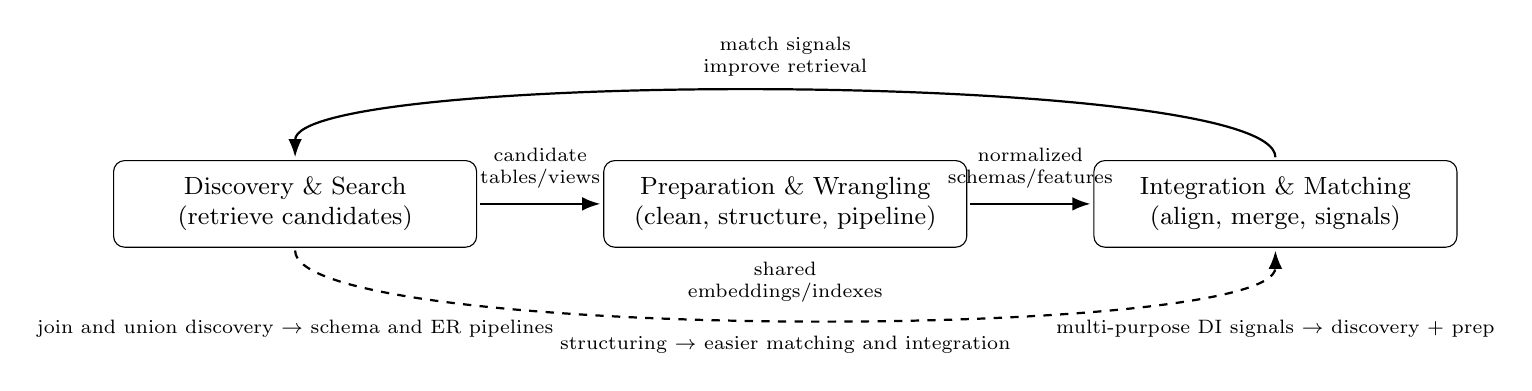
\begin{tikzpicture}[
  font=\small,
  phase/.style={
    draw,
    rounded corners,
    align=center,
    text width=4.4cm,
    minimum height=11mm,
    inner sep=3pt
  },
  arrow/.style={-Latex, thick, shorten <=1pt, shorten >=1pt},
  lbl/.style={font=\scriptsize, align=center}
]

\node[phase] (d) {Discovery \& Search\\(retrieve candidates)};
\node[phase, right=16mm of d] (p) {Preparation \& Wrangling\\(clean, structure, pipeline)};
\node[phase, right=16mm of p] (i) {Integration \& Matching\\(align, merge, signals)};

\draw[arrow] (d) -- node[midway, above=2pt, lbl]{candidate\\tables/views} (p);
\draw[arrow] (p) -- node[midway, above=2pt, lbl]{normalized\\schemas/features} (i);

\coordinate (upR) at ($(i.north)+(0,1.15cm)$);
\coordinate (upL) at ($(d.north)+(0,1.15cm)$);

\draw[arrow]
  (i.north) .. controls (upR) and (upL) .. (d.north)
  node[pos=0.5, above=2pt, lbl]{match signals\\improve retrieval};

\coordinate (dnL) at ($(d.south)+(0,-1.20cm)$);
\coordinate (dnR) at ($(i.south)+(0,-1.20cm)$);

\draw[arrow, dashed]
  (d.south) .. controls (dnL) and (dnR) .. (i.south)
  node[pos=0.5, above=2pt, lbl]{shared\\embeddings/indexes};

\node[below=8mm of d, lbl] {join and union discovery $\rightarrow$ schema and ER pipelines};
\node[below=10mm of p, lbl] {structuring $\rightarrow$ easier matching and integration};
\node[below=8mm of i, lbl] {multi-purpose DI signals $\rightarrow$ discovery + prep};

\end{tikzpicture}
\caption{Cross-phase dependencies. Many systems reuse representations, indexes, or learned signals across discovery, preparation, and integration.}
\label{fig:cross-phase-links}
\end{figure*}

\subsection{Phases Are Connected but Evaluation Is Isolated}
The three phases of a lake pipeline are tightly connected. Discovery controls which tables reach preparation and integration. Preparation changes how well those tables can be matched---for example, standardizing column formats makes later schema matching easier. End-to-end methods make these connections explicit by linking discovery, alignment, and integration in one workflow, or by reusing the same language model across discovery tasks \cite{10.1145/3555041.3589732,10.14778/3574245.3574274,10.14778/3659437.3659461,11112882}. Integration outputs (such as column matches and approximate key relationships) are also reused for retrieval and blocking, creating feedback loops \cite{10184556,10.1145/3588929}. Despite these connections, most methods report metrics for only one phase---for example, reporting retrieval precision without measuring whether the final merged table is correct. This can hide downstream problems: a discovery method with high precision may still retrieve tables that are hard to integrate. A practical lesson is to report stage-level results, maintenance cost, and at least one end-to-end outcome together.

Methods in different phases also optimize different goals---ranking quality, format consistency, or match accuracy---and without naming these differences, cross-method comparisons can look cleaner than they actually are.

\subsection{Ambiguity and User Intent}
In data lakes, ambiguity is unavoidable. Metadata is often missing or vague, and the same query can have many plausible answers. For example, searching for ``customer data'' might return sales records, support tickets, or demographic profiles---all valid depending on the analyst's goal. Discovery systems address this by supporting interactive refinement rather than assuming a single correct answer \cite{10184768,10.14778/3685800.3685880}. On the integration side, the same pair of records can be considered a ``match'' or ``non-match'' depending on the downstream task---FlexER~\cite{10.1145/3588722} demonstrates this with intent-aware entity resolution. This challenges the single-ground-truth assumption built into many benchmarks. An important open problem is \emph{intent-conditioned evaluation}: explicitly varying the analyst's goal and reporting how robust each method is across different intents and domains.

\subsection{Scalability, Cost, and Maintenance}
At the scale of real data lakes (thousands to millions of tables), major costs come from infrastructure: generating embeddings for every column, building and maintaining search indexes, and keeping everything up to date as new data arrives. End-to-end systems and benchmarks show why cost should be reported alongside effectiveness \cite{10.14778/3685800.3685880,10.14778/3659437.3659448,10.14778/3750601.3750694}. Preparation and integration face similar pressures: pipeline synthesis requires repeated execution, and progressive ER uses filtering and scheduling to control cost on a pay-as-you-go basis \cite{10.1145/3698831,10.1145/3709715,10184692}. Most current evaluations assume that the data does not change over time, which hides the real challenge of keeping results up to date as lake contents evolve. A key research direction is incremental maintenance---updating indexes, embeddings, and validation tests efficiently when new data arrives, rather than rebuilding everything from scratch.

\subsection{Preparation Needs Safety Checks}
Preparation can improve downstream quality, but improvements are not guaranteed. A repair system might over-edit---for example, ``correcting'' a valid but unusual value to something more common but wrong---or introduce plausible but incorrect values. Evaluation should therefore prioritize net error reduction (fixing more errors than the system introduces) and do-no-harm behavior \cite{10.14778/3675034.3675051}. Language-model-based curation adds further risks: models can hallucinate (generate plausible but fabricated values), give different answers on repeated runs (non-determinism), and expose private data if it is sent to an external API \cite{10.14778/3611540.3611624,10.14778/3574245.3574258}. Structuring methods also show that converting messy lake inputs into clean tables often requires multiple transformation steps, not just one \cite{10.1145/3665252.3665269,10.14778/3626292.3626294,10.14778/3681954.3682019}. In practice, systems need lightweight verification hooks---automated tests, constraint checks, and sample-based audits---that can trigger a rollback or request human review when confidence is low.

\subsection{Integration Design Choices}
Integration in data lakes is not as simple as ``match columns, then join.'' Real-world tables overlap only partially and have many missing values. Merge rules must therefore preserve partial facts while combining as much evidence as possible. For example, if Table~A has a customer's phone number but not their email, and Table~B has the email but not the phone, the merge should produce a row with both. Full Disjunction-style approaches show that careful merge operators can significantly outperform naive pairwise joins \cite{10.14778/3574245.3574274,10.1145/3555041.3589732}. At the entity level, workflow-oriented ER shows that the choice of blocking, scheduling, and supervision strategy often matters more for end-to-end performance and cost than the choice of matching model alone \cite{10.1145/3709715,10.1145/3588712,10.1145/3626711,10.1145/3588938}. Language-model-based matchers can reduce the need for labeled data and handle diverse formats, but they raise concerns about calibration (are the model's confidence scores reliable?), latency, and privacy \cite{10.14778/3742728.3742757}. A key open issue is choosing merge rules and workflow steps that align with the analyst's actual goal, and evaluating those trade-offs directly.

\subsection{Fairness, Privacy, and Governance}
As lake pipelines become more automated, responsible operation becomes part of system design, not an afterthought. Fairness-aware evaluation shows that overall accuracy can mask unequal error rates across groups---for example, an entity-matching system may work well for common names but poorly for uncommon ones \cite{10.14778/3611479.3611525}. Language-model-based data tasks also raise privacy risks: converting data into text prompts and sending them to an external API can leak sensitive information or violate organizational policies \cite{10.14778/3574245.3574258}. Governance rules---organizational policies about which tables can be joined, which attributes can be exposed, and which external sources can be used---should be built into the pipeline as planning constraints, not checked only after the fact. Open problems include auditing fairness at every stage (not just the final matcher), developing privacy-preserving indexing and language-model techniques, and building integration planners that respect organizational policies by design.

\subsection{Benchmark Gaps and Shared Test Collections}
Shared corpora and benchmarks have improved comparability within each phase: GitTables~\cite{10.1145/3588710} and LakeBench~\cite{10.14778/3659437.3659448} standardize parts of discovery evaluation, and ER benchmarks support workflow comparison \cite{10184692}. Learned embeddings and profiling signals are also reused across tasks \cite{10184556,10.1145/3588929}. However, few resources cover the full pipeline---discovery through preparation through integration---under realistic conditions such as data updates, changing analyst intent, and explicit cost reporting. A concrete next step is a pipeline test collection that combines workloads from all three phases, provides ground truth at each stage, and tracks computational cost (Table~\ref{tab:benchmark_inventory}).

% ---- Benchmark inventory table ----
\begin{table*}[!htbp]
\centering
\caption{Inventory of shared resources and the gaps they suggest.}
\label{tab:benchmark_inventory}
\tbl
\begin{tabularx}{\textwidth}{@{}p{26mm}p{26mm}Y Y@{}}
\toprule
\textbf{Artifact} & \textbf{Phase(s)} & \textbf{What it enables} & \textbf{Key gaps / limitations} \\
\midrule
GitTables~\cite{10.1145/3588710} &
Discovery (rep.\ learning) &
Large table corpus for training/evaluation of semantic table understanding and retrieval &
Limited evolving-lake settings; not a full end-to-end pipeline workload. \\
\addlinespace[0.25em]
LakeBench~\cite{10.14778/3659437.3659448} &
Discovery (join and union) &
Join/union discovery benchmarks with labeled queries; effectiveness+efficiency comparisons &
Mostly stage-local; limited coupling to preparation/integration outcomes. \\
\addlinespace[0.25em]
Filtering/ER benchmarks~\cite{10184692} &
Integration (ER workflows) &
Systematic evaluation of filtering and scheduling configurations and trade-offs &
Fairness/intent labels are rare; limited policy constraints and multimodal settings. \\
\addlinespace[0.25em]
Reusable signals~\cite{10184556,10.1145/3588929} &
Cross-phase &
Shared representations and profiling signals transferable across tasks &
Need standardized reporting of cost, calibration, and behavior under updates/shift. \\
\bottomrule
\end{tabularx}
\end{table*}

Such a test collection is especially useful because failures often occur at the boundaries between phases---for example, discovery returning structurally incompatible tables, or preparation removing values needed for later matching.

\subsection{Threats to Validity}
This study has limits. We searched three venues (SIGMOD, PVLDB, ICDE), so methods published elsewhere may be missing. Some methods could fit more than one category; we mitigate this by assigning each to exactly one phase based on its primary output. The 2022--2025 window narrows our view; earlier work is cited but not covered in the same depth. Methods across phases optimize different goals (ranking quality, consistency, match accuracy), so side-by-side comparison is inherently imperfect. Limited code and data release makes full reproducibility difficult. We keep phase-specific metrics separate and note where reproducibility is weak.

\subsection{Research Agenda}
Five concrete next steps emerge:
(1)~\textbf{End-to-end discovery evaluation}---report downstream integration quality, not only ranking metrics.
(2)~\textbf{Joint preparation evaluation}---measure both local repair quality and downstream utility on the same tables.
(3)~\textbf{Integrated integration metrics}---report pairwise match accuracy alongside final-table completeness.
(4)~\textbf{Update-aware studies}---test workflows on time-sliced lake snapshots to measure quality drift and maintenance cost.
(5)~\textbf{Cross-phase fairness and privacy audits}---audit all three phases under one protocol with subgroup definitions and policy rules.

% ==========================================================
\section{Conclusion}
% ==========================================================
We reviewed 49 methods from 2022--2025 across discovery, preparation, and integration. Three patterns recur: discovery increasingly combines embeddings with practical indexing; preparation increasingly produces repeatable automated workflows but still needs safety checks; and integration increasingly depends on workflow design and analyst intent rather than a single matching score. A natural next step is pipeline-aware evaluation: shared test collections that connect stage-level results to end-to-end outcomes under realistic conditions including data updates, ambiguous intent, and explicit cost measurement.


% ==========================================================
\balance
\bibliographystyle{ACM-Reference-Format}
\bibliography{ref}
% ==========================================================

\end{document}
